The \emph{SafeStreets} system can be viewed as a standalone system in the sense that it does not depend on other external systems in order to properly function. However, in order to provide some external services to other entities it requires the provision communication interfaces to facilitate the flow data to and from the system. To be more specific, to interact with the municipality it is needed to have the appropriate interfaces as channels to retrieve data to be processed and to provide processed and aggregated data.

Apart from the aforementioned system interaction, \emph{Safastreets} seldom depends on external services or systems. This is specially true for the main features of the system; i.e., the services provided to the civilian users. Specifically, the service provided in order for users to report traffic violations and the \emph{View Safety} feature which could be seen to built upon the first feature; since, it is considered as a geographically oriented representation of report data.

Surely, the internal modules of the system are codependent since the data collected from user and possibly retrieved from the authorities flows internally through the system in many forms such as raw report details, insights built on report details and graphical representations. \emph{Figure 1} provides a high level representation of the entities interacting with the system and represents the relationship between abstract entities, such as, \emph{Report} and \emph{Safety Representation}.
\newpage

***place holder for entity class diagram***

\newpage
Furthermore, since the users are viewed as the main entity interacting with the \emph{Safestreets} system it is rather important to clearly define the different states of the user and the state defining interactions with the system. First and foremost, it is worthy of mention that all user-system interactions are done through the user interfaces to be presented in the following sections. Moving onto the relevant topic of user states as seen by the system, any user can be classified into one of three categories; this classification is based on the different features accessible to the user. First, is the \emph{unregistered users} who are unable to access any of the system features until registration; which brings us to the second category of user, the registered users which are able to access all system features apart from creating traffic reports; atleast, not until they allow the system to access their mobile phone camera and location services. Finally, fully activated users who have are able to fully exploit the \emph{SafeStreets} features.

The following state diagrams show a clear representation of the different user states and the user actions that cause a transition from one classification to another. As well as, a representation of the permission granting process that is a sort of a prerequisite for becoming an activated user.



\begin{figure}[H]
\caption{Sequence diagram for Login}
\label{fig:SD-login}
\centering
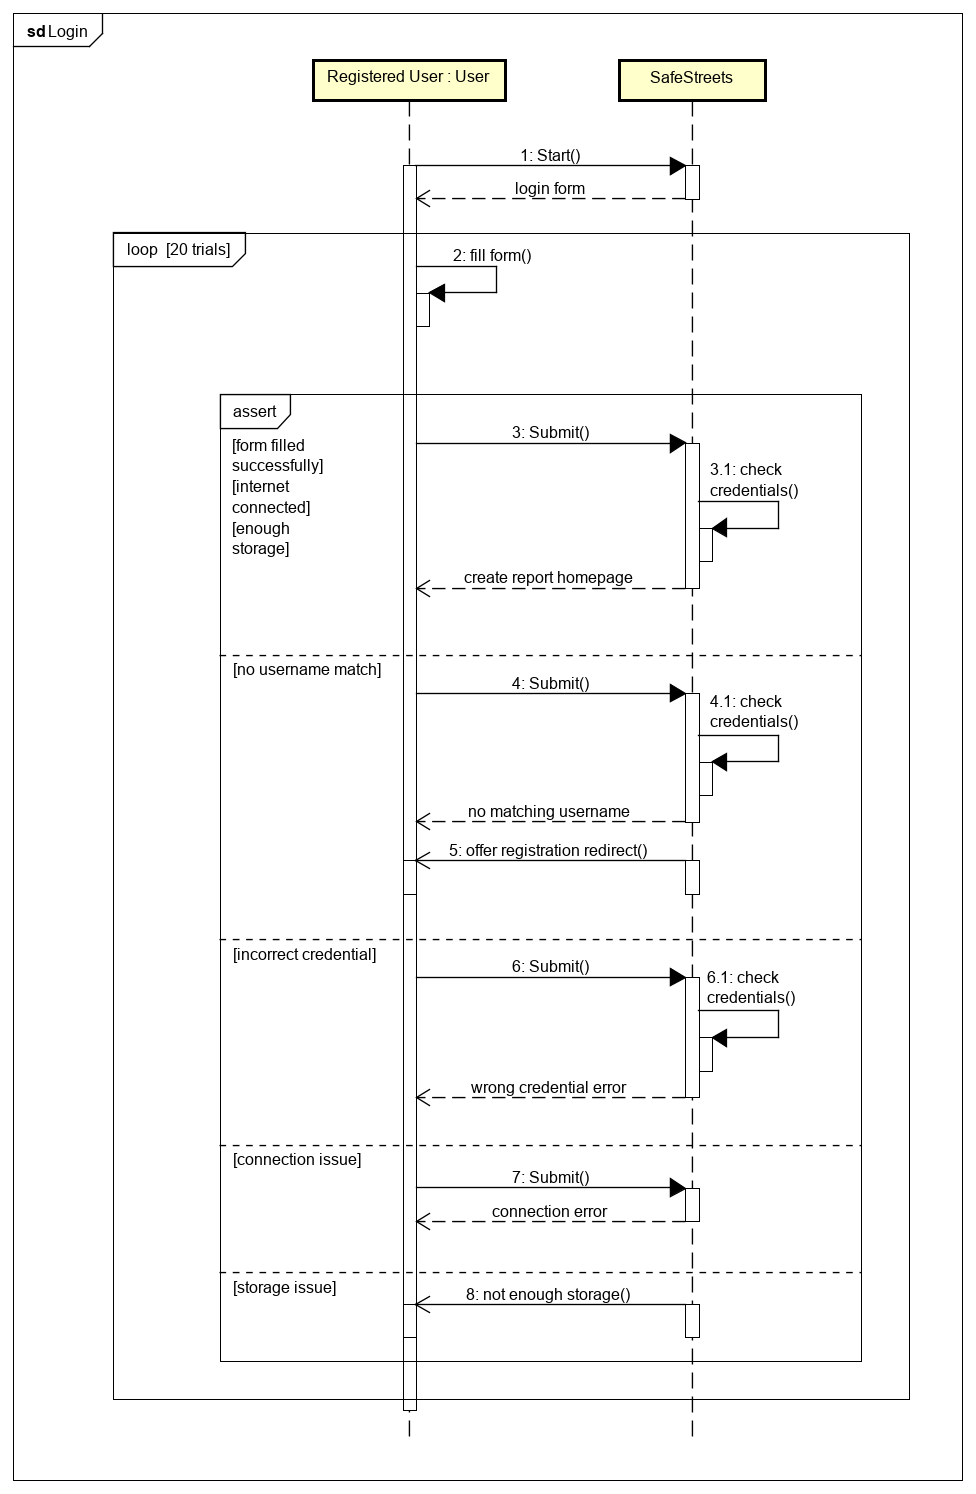
\includegraphics[width=\textwidth, height=\textheight]{login-SD.png}
\end{figure}

